%%%%%%%%%%%%%%%%%%%%%%%%%%%%%%%%%%%%%%%%%%%%%%%%%%%%%%%%%%%%%%%%%%%%
\chapter{Guiding principles of the code}
\label{ch:philosophy}

\ds\ (as of version 6) has a new structure compared to earlier versions of the code. The most 
striking difference is that we have split the particle physics model dependent parts from 
the rest of the code. This means in practice that we have separated \ds\ into one set of 
routines, \code{ds\_core}, which contains no reference to any specific particle model, as 
well as distinct sets of routines for each implemented model of particle physics. For 
supersymmetry, 
 for example, all routines that require model-dependent information now reside in the 
 \code{mssm} module. The advantage with this setup is that \code{ds\_core} and the 
 particle physics modules may be put in separate FORTRAN libraries, which implies
 that \ds\ can now have several particle physics modules side by side. The user 
 then simply decides at the linking stage, i.e.~when making the main program, which 
 particle physics module to include. 
 
 For this to work, the main library communicates with the particle physics modules via
 so-called \emph{interface} functions (or subroutines), with 
 pre-defined signatures and functionalities.  Note that a 
 particle physics module does not have to provide all of these predefined functions: 
 which of them are required is ultimately determined only when the user links the main
 program to the (\code{ds\_core} and particle module) libraries. Assume for example that 
 the main program wants to calculate 
 the gamma-ray flux from DM (a functionality provided by \code{ds\_core}). This is only
 possible if the particle module provides an interface function for the local cosmic ray
 source function; if it does not, the main program will not compile and a  
 warning is issued that points to the missing interface function. If, on the other hand,
 interface functions required by direct detection routines would be missing in this example,
 this would not create any problems at either runtime or the compile stage.


 In addition, we have added the concept of 
 \emph{replaceable functions}, which allows users to replace essentially any function in 
 \ds\ with a user-supplied version. \ds\ ships with dedicated tools to assist you setting up 
 both replaceable functions and new particle physics modules.
 Fig.~\ref{fig:concept} illustrates these concepts by showing how a typical program 
 would use \ds; below, we describe each of them in more detail. 

%%%%%%%%%%%%%%%%%%%%%%%%%
\begin{figure}[t!]
\centering
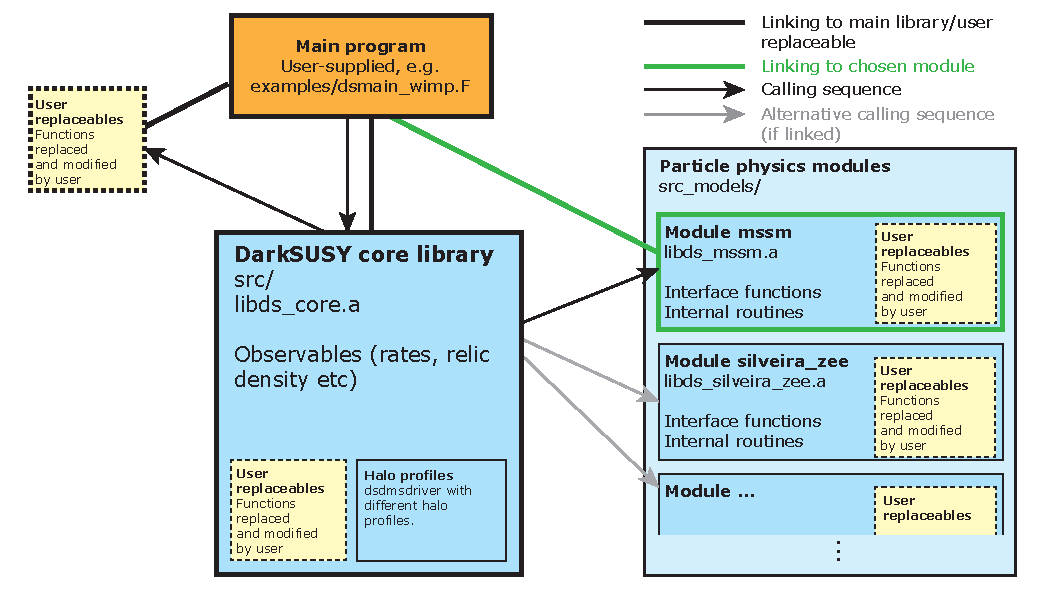
\includegraphics[width=\textwidth]{fig/ds6-structure-v6}
\vspace{-0.5cm}
\caption{Conceptual illustration of how to use \ds. The main program links
to both  the main library, \code{ds\_core}, and to \emph{one} of the available particle 
physics modules. User-replaceable functions are optional and may be linked to directly 
from the main program, or indirectly by including them in the various libraries. 
See \code{examples/dsmain\_wimp.F} for an example of a main program that demonstrates
typical usage of \ds\ for different particle physics modules.}
\label{fig:concept}
\end{figure}
%%%%%%%%%%%%%%%%%%%%%%%%%%		


%%%%%%%%%%%%%%%%%%%%%%%%%%
\begin{table}[t!]
%\centering
%\begin{tabular}[l]{l|l}
%subdirectory name & description\\
%\hline
%\code{src/ini} & Initialization routines\\
%\code{src/ge} & General utility functions of the main library\\[1ex]
%
%\code{src/an\_yield} & Simulated yield tables, e.g.~from $\bar bb$ final states\\
%\code{src/cr\_axi} & (Anti-)nucleon propagation routines for a generic 
%                               \\&axially symmetric diffusive halo\\
%\code{src/cr\_dmd} & Dark matter density profiles\\
%\code{src/cr\_gamma} & Gamma-ray routines, line-of-sight integrations etc.\\
%\code{src/cr\_ge} & general, auxiliary functions needed by cosmic ray routines\\
%\code{src/cr\_ps} & Positron propagation routines\\[1ex]
%
%\code{src/se\_aux} & Auxiliary routines needed by capture rate routines\\
%\code{src/se\_yield}& Simulated neutrino yield tables from the center of the Sun or Earth\\
%\code{src/se\_ic}& Neutrino flux likelihood calculations, using IceCube data\\
%\code{src/se\_mod} & Density and composition models for the Sun and the
%Earth\\
%\code{src/se\_nu} & Capture rate for dark matter in the Sun and in the Earth,
%\\& as well as neutrino fluxes from the center of Sun and Earth\\[1ex]
%
%\code{src/dd} & Direct detection routines\\[1ex]
%
%\code{src/kd} & Kinetic decoupling\\
%\code{src/rd} & Relic density\\[1ex]
%
%\code{src/xCERN} & numerical routines from the CERN library \cite{?} \\
%\code{src/x...} & Other contributed external code 
%            \\ & (currently \code{cmlib} \cite{?}, \code{diag} \cite{?} and \cod%e{galprop} \cite{?})\\
%\end{tabular}
[SRCLIST]
\caption{Organization of the main library  \code{ds\_core}: all functions and subroutines 
reside in the \code{src/} folder of the \ds\ installation, with the names of the subdirectories 
indicating the subject area. (Note: this table is automatically generated from the actual directory structure in \code{src/}.)
}
\label{tab:dsmain}
\end{table}
%%%%%%%%%%%%%%%%%%%%%%%%%%		


\section{The main \ds\ library \code{ds\_core}}

\index[routines]{ds\_core} As introduced above, the main library is in some sense the heart of the new \ds\,,
offering all the functionality that a user typically would be interested in without having 
explicitly to refer to specific characteristics of a given particle physics model (after
initialization of such a model).
 The main library thus contains routines for, e.g., 
cosmic ray propagation, solar models, capture rates for the Sun/Earth, a 
Boltzmann solver for the relic density calculation, yield tables from annihilation/decay etc. 
None of the routines in the main library contains any information about the particle 
physics module. Instead any information needed is obtained by calling a required 
function that resides in the  particle physics module which is linked to (see below). 

The source code for all functions and subroutines in the main library can be found in the 
\code{src/} directory of the \ds\ installation folder, with subdirectory names indicating  
subject areas as summarized in Table \ref{tab:dsmain}.


%%%%%%%%%%%%%%%%%%%%%%%%%%%%%%%%%%%%%%%%%%%%%%%%%%%%%%%%%%
%%%%%%%%%%%%%%%%%%%%%%%%%%%%%%%%%%%%%%%%%%%%%%%%%%%%%%%%%%
\section{Particle physics modules}
\label{sec:particle_modules}

\index{particle physics modules} The particle physics modules contain the parts of the code that 
depend on the respective 
particle physics model. Examples are cross section calculations, yield calculations etc. 
The routines in the particle physics module have access to all routines in 
\code{ds\_core}, whereas the reverse is in general not true (with the exception of a very limited 
set of interface functions that each particle module provides). 

\ds\ 5 and earlier was primarily used for supersymmetric, and neutralino DM, and those 
parts of the code now reside in the MSSM module \code{mssm}. However, many people 
used \ds\ even before for e.g.\ a generic WIMP setup, which was doable for parts of the 
code, but not all of it. We now provide a generic WIMP module \code{generic\_wimp} that 
can be used for these kinds of calculations in a much more general way. 
 In a similar spirit,
we also provide a module \code{generic\_decayingDM} for phenomenological studies
of decaying DM scenarios. As an example for an actual particle physics model
other than supersymmetry,
\ds\  furthermore includes a module \code{silveira\_zee} which implements the
DM candidate originally proposed by Silveira and Zee \cite{Silveira:1985rk} and which 
now is often
referred to as Scalar Singlet DM \cite{McDonald:1993ex,Burgess:2000yq,Cline:2013gha}.
%We also provide a module for universal extra dimensions, \code{ued}. It is far from complete, 
%as of version 6 of the code, but serves to illustrate that even if you do 
% not have the complete module, you can still use \ds\ for calculations where your module 
% provides required functions beyond simple dummy versions.
We also include an empty model, \code{empty}, 
which is of course not doing any real calculations, but contains (empty versions of) all
interface functions that the core library is aware of -- which is very useful for debugging and
testing purposes. Designing new particle modules is 
a straight-forward exercise, see below, and it is generally a good idea 
to start with the most similar module that is already available.

A list of the currently available particle physics modules is given in table~\ref{tab:modules},
and the source code for the particle modules can be found in the \code{src\_models/} 
directory of the \ds\ installation folder, each of the subdirectories 
(e.g.~\code{src\_models/mssm/}, \code{src\_models/generic\_wimp/}) typically 
reflecting a (sub)subdirectory structure analogous to what is shown in Table \ref{tab:dsmain}
for the core library. 
%
Many dark matter models, furthermore, constitute only relatively simple extensions to the 
standard model, inheriting most of its structure. For convenience,
we therefore also provide various auxiliary routines, in \code{src\_models/common/sm}, that each particle module 
automatically has access to, and which return basic standard model quantities like, e.g., the masses
of standard model particles and their running (so additional BSM effects have to be implemented in the
respective particle module).


\begin{table}[t!]
[MODULESLIST]
\caption{List of particle physics modules currently available in \code{src\_models}. (Note: this table is automatically generated from the actual content of \code{src\_models}.)}
\label{tab:modules}
\end{table}


\subsection{Using a particle physics module}
%%%%%%%%%%%%%%%%%%%%%%%%%%%%%%%%%%%%%%%%%%%%%%%%%%%%%%%%%%%%%%%%%%%%

How to use a particle physics module obviously depends on how it is implemented,
and in principle there are no formal requirements on how this should be done -- as long as the 
provided interface functions are correctly set up, see Section \ref{sec:interface} further down.
The one subroutine that {\it is} required to exist, however, is
\begin{verbatim}
dsinit_module
\end{verbatim}
This is called directly from \code{dsinit}, and must be the first call to the particle module 
as it initializes all general settings and relevant common block variables. 

While there is no required structure otherwise, there is a typical workflow associated to using
a particle physics module in a main program. First, one needs to initialize a given model
by specifying its model parameters. This is done by routines like
\begin{verbatim}
dsgivemodel...
\end{verbatim}
A call to \code{dsgivemodel\_decayingDM}, e.g., allows to enter the defining parameters for 
a DM model in the \code{generic\_decayingDM} module, while \code{dsgivemodel\_25} allows 
to enter the parameters for pMSSM model with 25 parameters in the \code{mssm} module.
The next step is then typically a call to
\begin{verbatim}
dsmodelsetup
\end{verbatim}
in order to transfer the model parameters to common blocks and calculate basic quantities like
masses and couplings. Once a model is set up like this, a main program can use the full
functionality of \ds\ supported by the respective module.


\subsection{Adding a new particle physics module}


To create a new particle physics module, the easiest way is to start from an existing one as a template 
and create a new one from that one. To help you in this process we provide a script 
\code{scr/make\_module.pl} that takes two arguments, the module you want to start from and 
the new one you 
want to create (for further instructions, just call the script without arguments). 
It will then copy the module to a new one, change its name 
throughout the module and make sure that it is compiled by the makefiles and included properly when 
requested by the main programs. If you specify the option \code{-i} only interface functions will be copied 
(which creates a cleaner starting point, but also will most likely not compile without modifications). When 
creating a new module this way, the best is to copy from a module that is as similar as possible to your 
new model. If you want a clean setup, you can always copy from the \code{empty} module. If you want something more phenomenological that has a basic framework for calculating observables, starting from the \code{generic\_wimp} or \code{generic\_decayingDM} might be a good idea. A general
advice is to view the modules we provide as a starting point as inspiration for your new modules.

Even though a particle physics module does not need to include all interface functions (which ones 
are needed only depends on the observables you try to calculate in your main programs), it needs to provide 
an initialization routine 
\code{dsinit\_module.f}. This routine should set a global variable \code{moduletag} to the name of 
the module so that routines that need to check if the correct module is loaded can do so. When using the 
script \code{scr/make\_module.pl} this routine is always created and \code{moduletag} set as it should.


Note that the script \code{scr/make\_module.pl} only provides the framework in the configure script and makefiles (or rather makefile.in's) to make sure your module is compiled. It does \emph{not} create a main program that uses your module, that is up to you. A good starting point for that can either be e.g.\ \code{dsmain\_wimp.F} in examples that already contain different blocks for different modules (controlled by pre-compiler directives, see the code for more details). Another option is to use any of the example programs in \code{examples/aux} as a starting point. 

To make upgrading to new \ds\ versions as smooth as possible, we advice to create your own folder with your main programs, using e.g.\ the \code{makefile} in \code{examples/aux} as a starting point. Don't modify any of the \ds\ \code{makefile}s directly as they are overwritten every time you run \code{configure}, see Section~\ref{sec:makeownmain} for more details.

Note that for the \code{scr/make\_module.pl} script to work you need to have \code{autoconf} installed as the script adds your new module to \code{configure.ac} and runs \code{autoconf} to create a new \code{configure} script.

%%%%%%%%%%%%%%%%%%%%%%%%%%%%%%%%%%%%%%%%%%%%%%%%%%%%%%%%%%
%%%%%%%%%%%%%%%%%%%%%%%%%%%%%%%%%%%%%%%%%%%%%%%%%%%%%%%%%%
\section{Halo models}
\label{sec:halo_general}

Several routines in the core library need to know which DM halo should be adopted for the 
calculations. With this \ds\ version, we introduce a new and flexible scheme that avoids 
pre-defined hardcoded functions to describe the DM density profiles, and allows to 
consistently define different DM targets at the same time. For convenience, we still provide
several pre-defined options for such halo parameterizations, and the user can choose 
between, e.g., the Einasto \cite{1965TrAlm...5...87E} and the Navarrow-Frenk-White profile 
\cite{Navarro:1995iw}, or read in any tabulated axi-symmetric (or spherically symmetric) profile. 
On a {\it technical} level, the halo models are handled by the \code{dsdmsdriver} routine which 
contains a database of which  halo profiles the user has set up, and consistently passes this
information to all parts in the code where it is needed.\footnote{
From a technical point of view, it is actually not  \code{dsdmsdriver} itself which acts as an interface
to the rest of the code, but the set of wrapper routines collected in \code{src/dmd\_astro} (which all call \code{dsdmsdriver}
in a specific way). Only those routines are called by 
cosmic-ray flux routines and other functions in \code{src}, never \code{dsdmsdriver} directly.
The routines in  \code{src/dmd\_astro} therefore provide examples of functions that {\it cannot be
replaced} individually in a consistent way, but only as a whole set (along with \code{dsdmsdriver},
in case the user wants to change the structure of the driver itself).  
} 

We provide detailed hands-on examples on how to use this system by a set of example
programs \code{DMhalo\_*.f}, see Section \ref{sec:aux_ex}. For further details, we refer
to Section \ref{sec:halo} of this manual.


%%%%%%%%%%%%%%%%%%%%%%%%%%%%%%%%%%%%%%%%%%%%%%%%%%%%%%%%%%
%%%%%%%%%%%%%%%%%%%%%%%%%%%%%%%%%%%%%%%%%%%%%%%%%%%%%%%%%%
\section{Interface functions}
\label{sec:interface}

\index{interface functions} Interface functions are functions that routines in \code{ds\_core} might need to call, and
which therefore every particle physics module should contain if that particular observable is requested. 
Examples of interface functions include \code{dsddsigma} that returns the equivalent DM nucleus cross section, \code{dscrsource} that 
returns the source term for DM-induced cosmic rays (relevant for indirect detection),
\code{dsanxw} that returns the invariant annihilation rate (in the case of WIMPs), etc.
 All interface functions are found by looking in the empty module, and always contain the 
 keyword `interface' in the function or subroutine header.

If a particle physics module contains the full set of interface functions, all
routines in the main \ds\ code should work. However, this is not needed to set up a paticle physics module. E.g.\ a generic WIMP model does not need to have decay rates set up. If a routine in the main \ds\ routines is called that rely on this interface being present, an error will be thrown when trying to compile your code. This of course applies to all interface functions, not just unphysical ones. E.g.\ if you are only interested in the relic density for a new particle physics module, you do not need to set up scattering rates, cosmic ray source functions, etc.

In Tab.~\ref{tab:if}, we provide the complete list of interface functions currently implemented in \ds,
along with a brief description. For more details, consult the headers of these files.

\bigskip

\begin{table}[!h]
[IFLIST]
\caption{Table of interface functions, which modules that contain them (with numbering from table~\ref{tab:modules}, where they are used and a short description of them. (Note: this table is automatically generated from scanning through the particle physics modules in \code{src\_models}. The description is taken from the \code{empty} module routine headers.)}
\label{tab:if}
\end{table}


%%%%%%%%%%%%%%%%%%%%%%%%%%%%%%%%%%%%%%%%%%%%%%%%%%%%%%%%%%
%%%%%%%%%%%%%%%%%%%%%%%%%%%%%%%%%%%%%%%%%%%%%%%%%%%%%%%%%%
\section{Commonly used functions}

\index{commonly used functions}Routines that we believe are particularly  useful for most users to call, we denote 
as \emph{commonly used functions}. A list of the commonly used functions in the main \ds\ library in \code{src} is 
shown in Table \ref{tab:culist}. The routines are described in more detail in their corresponding chapters in part II of 
this manual, as indicated in the table \ref{tab:culist}. 

\bigskip

\begin{table}[!h]
[CULIST]
\caption{List of commonly used functions and subroutines. (Note: this table is automatically generated from the routines in \code{src} that have the commonly used tag in their header.)}
\label{tab:culist}
\end{table}


\section{Replaceable functions}
\label{sec:replaceable}
\index{replaceable functions}
The concept of replaceable functions introduces the possibility to replace a \ds\ routine with one of your own. The way it works is that the user-provided function will be linked 
when you make your main program instead of the \ds\ default one. If, for example, you want to 
replace the yields from a typical final state of DM annihilation or decay (like $\bar bb$)
with a new function of your own -- e.g.~because you are interested in comparing the tabulated
{\sf Pythia} \cite{Sjostrand:2006za} yields with those provided by PPPC \cite{Cirelli:2010xx} --  
you create your own version of the routine \code{dsanyield\_sim} and let \ds\ use this one 
instead.  To help you with this setup, 
we provide tools that can create (or delete) a replaceable function from any \ds\ function 
and set up the makefiles to use this user-supplied function instead. We also provide a
simply way of managing large `libraries' of user-supplied functions, via a list imported 
by the makefiles, where the user can determine on the fly which user-replaceable 
functions should be included and which ones should not.  Note that both routines in 
\code{ds\_core} and in any of the particle physics modules can be replaced in this way,
including interface functions. There is also a possibility for the particle physics modules to replace a
function in the core library. This is not used often, but is used e.g.\ for the function \code{dsrdxi.f} (which gives a possibility to have different dark matter and background temperatures in the early Universe).

There is also a simple way to bypass this system  -- indicated in the left-most part of Fig.~\ref{fig:concept} --
by directly linking to the user-supplied function only when making the main program. 
 For an explicit example, see (the makefile for) \code{generic\_wimp\_oh2.f}.

